%%%%%%%%%%%%%%%%%%%%%%%%%%%%%%%%%%%%%%%%%%%%%%%%%%%%%%%%%%%%%
% Use the BCUDissertation class
%%%%%%%%%%%%%%%%%%%%%%%%%%%%%%%%%%%%%%%%%%%%%%%%%%%%%%%%%%%%%
\documentclass{BCUDissertation}

% Adding multiple bibliography's
% References.bib and Bibliography.bib
% References: Used for cited references
% Bibliography: used for papers read but not cited
\newcites{bibs}{Bibliography}

%%%%%%%%%%%%%%%%%%%%%%%%%%%%%%%%%%%%%%%%%%%%%%%%%%%%%%%%%%%%%
% Enter document details here
%%%%%%%%%%%%%%%%%%%%%%%%%%%%%%%%%%%%%%%%%%%%%%%%%%%%%%%%%%%%%
\author{Harvey Fretwell}
\title{Comparative Analysis of Auto Phase Alignment Techniques: Traditional DSP Methods VS. Neural Network Approaches}
\course{Sound Engineering and Production}
\department{School of Computing and Digital Technology}
\date{\todo{Month} 2023}

%%%%%%%%%%%%%%%%%%%%%%%%%%%%%%%%%%%%%%%%%%%%%%%%%%%%%%%%%%%%%
% Define acronyms
%%%%%%%%%%%%%%%%%%%%%%%%%%%%%%%%%%%%%%%%%%%%%%%%%%%%%%%%%%%%%
% Acronyms are defined using the \newacronym command.
%  * The first argument is the name of the acronym.
%  * The second argument is the abbreviated form.
%  * The third argument is the full form.
\newacronym{tla}{TLA}{Three Letter Acronym}
\newacronym{wysiwyg}{WYSIWYG}{What You See is What You Get}
\glsfindwidesttoplevelname % Leave this here so the list of acronyms looks nice

%%%%%%%%%%%%%%%%%%%%%%%%%%%%%%%%%%%%%%%%%%%%%%%%%%%%%%%%%%%%%
% Begin the document.
%%%%%%%%%%%%%%%%%%%%%%%%%%%%%%%%%%%%%%%%%%%%%%%%%%%%%%%%%%%%%
\begin{document}

%%%%%%%%%%%%%%%%%%%%%%%%%%%%%%%%%%%%%%%%%%%%%%%%%%%%%%%%%%%%%
% Create title page.
%%%%%%%%%%%%%%%%%%%%%%%%%%%%%%%%%%%%%%%%%%%%%%%%%%%%%%%%%%%%%
\maketitle

%%%%%%%%%%%%%%%%%%%%%%%%%%%%%%%%%%%%%%%%%%%%%%%%%%%%%%%%%%%%%
% Set initial page numbering to be lower case roman numerals and include the contents of the preamble.tex file.
%%%%%%%%%%%%%%%%%%%%%%%%%%%%%%%%%%%%%%%%%%%%%%%%%%%%%%%%%%%%%
% Leave this here to use roman numeral page numbering for the preamble.
\pagenumbering{roman}

% The Abstract
\begin{abstract}
	\note{
	    A summary of the report (100-300 words), which should fully encapsulate the content of the project, while being informative, interesting and contain appropriate quantitative aspects (e.g., results). It should describe the project in one paragraph to follow introduction, method, results and conclusion. An example is provided below.
	    
	    Example:
	    
	    Automated drum transcription (ADT) systems attempt to generate a symbolic music notation for percussive instruments in audio recordings. Neural networks have already been shown to perform well in fields related to ADT such as source separation and onset detection due to their utilisation of time-series data in classification. An ADT system based on neural networks is proposed in order to exploit their ability to capture a complex configuration of features associated with individual or combined drum classes. In this paper, a bi-directional recurrent neural network is proposed for offline detection of percussive onsets from specified drum classes and a recurrent neural network suitable for online operation. In both systems, a separate network is trained to identify onsets for each drum class under observation—that is, kick drum, snare drum, hi-hats, and combinations thereof. Four evaluations are performed utilising the IDMT-SMT-Drums and ENST minus one datasets, which cover solo percussion and polyphonic audio respectively. The results demonstrate the effectiveness of the presented methods for solo percussion and a capacity for identifying snare drums, which are historically the most difficult drum class to detect.
	}
\end{abstract}

% Acknowledgements
\begin{acknowledgements}
	\note{
        Identifying those from whom assistance has been received. Use discretion in selecting the most relevant people who have directly helped or influenced the project completion.
        
        Example: 
        
        First and foremost, I would like to thank my advisor, Prof. Charles Xavier, for his supervision throughout the course of my doctoral studies at Birmingham City University. Prof. Xavier has tirelessly provided his encouragement and guidance, which has helped me to define my research goals and to shape the scope and focus of this dissertation. His suggestions and careful critique during all stages of this dissertation were indispensible to the creation of this document. In this regard, I would also like to thank Dr. Jean Grey for her detailed reading and guidance towards a more cohesive, structurally-sound work. I very much appreciate the thoughtful reading and suggestions for improvements and future work provided by Dr. Hank McCoy, Piotr Rasputin, and Ororo Munroe.

	}
\end{acknowledgements}

% ToC and lists of figures/tables etc.
\tableofcontents
\listoffigures
\listoftables
\listofacronyms
\clearpage

%%%%%%%%%%%%%%%%%%%%%%%%%%%%%%%%%%%%%%%%%%%%%%%%%%%%%%%%%%%%%
% Set page numbering back to normal numbers and include each individual chapter.
%%%%%%%%%%%%%%%%%%%%%%%%%%%%%%%%%%%%%%%%%%%%%%%%%%%%%%%%%%%%%
% Leave these here to change back to normal page numbering and add some nice headers to the pages.
\pagenumbering{arabic}
\pagestyle{headings}

\section{Introduction}
    \note{
        This will clearly state the rationale and objectives of the research and contain much of the same information present in the proposal (e.g., problem definition, scope, rationale, aims and objectives). Begin with a brief introduction to provide preparation for the rest of the report, with a clear outline of what was done and the rationale for the work. Much of the information that you have already written will be utilised throughout this section, however it should be specifically tailored to this assessment point.
    
        Start the introduction by answering the question: What is the subject of the project?
    }
    
    \subsection{Aims}
        \note{
            There should be a brief and precise statement of overall aim—what is intended to be attained?
        }
    
    \subsection{Objectives}
        \note{
            There should follow a list, using bullet points, of objectives—the completion of which will lead to the attainment of the aim. The objectives are developed from the aim and can be viewed as incremental stages in the attainment of the aim(s). Bloom’s Taxonomy is useful in writing these objectives (see Moodle site).
        }
        \begin{itemize}
            \item One
            \item Two
            \item Three
            \item Four
            \item Five
        \end{itemize}
    
\section{Literature Review}
    \note{This is an organised, critical report detailing the various sources of applicable research around relevant topics. Note that this is an indicative example of the report structure that should be used. Refer to the Project Handbook (p. 18-20) and video tutorials in weeks 4-7 for an explanation of content to be included. This should be discussed with your supervisor well in advance, as subject areas may have different approaches that are not in line with the one presented here. The literature review should be approximately 2000 words.}
	
    \subsection{Themes}
        \note{Discuss what areas (i.e., themes) need to be explored and why. Typically, there will be around 5 or 6 themes required. You may refer to a mind map in the Appendix showing themes if it helps (but this is not necessary). State the keywords used, which are associated with each theme. Example phrasing: 'A thematic approach has been undertaken to identify the areas that need to be understood to develop the artefact. From this, a number of keywords for each have been used to obtain information from the literature'. List your themes and give example keywords. Note that one of the themes to consider in the literature review is how other researchers approach the topic of evaluation.}
        
    \subsection{Review of Literature}
        \note{This subsection will comprise the main body of the literature review. It will contain a historical overview of the literature relevant to each theme in your project. Relational information about each reference will be presented to provide context for various sources (i.e., brief description of important aspect(s) of each source) and a system of categorisation of topics (i.e., modes of interpreting sources) will be used to separate sources into different classes. This can either be written as one subsection for each theme or as two subsections (i.e., Review and Theory) for each theme as below. If one subsection is used, the information in the Review and Theory sections below must be woven together for each theme discussed. This means you will have one subsection for each theme. This will be determined through discussion with your supervisor.}

    \subsubsection{Review}
        \note{Should be who did what and why for each theme. While this is a critique, it is NOT your opinion on research undertaken by other researchers. It must include many citations for each theme (at least 8 references for each theme) and a useful ordering of information is based a timeline in years. This is NOT a description of a paper or article in a list format.}

    \subsubsection{Theory}
        \note{Details of how things work. This is very different from the Review, which provides cursory links between research. It should include design methods (e.g., equations, algorithms) that will be used and so on. There is no need to start from basics (e.g., V=IR, syntax error) as the reader will have some knowledge.}

    \subsection{Summary}
        \note{Provide an overview of the topics discussed and information presented. Given this information that you have read, what conclusions may be drawn from this? How does this lead into the choices made going into the following section?}

\section{Method and Implementation}
    \note{
        This section describes the development of the artefact, including design and implementation. This should be derived from your previous design and methods report. This should be an updated version, which reflects the progress made in the implementation along with feedback from your supervisor.
        
        Remember that success of the project depends upon careful selection of appropriate method (e.g., design, model). A good method increases the validity and reliability of the outcomes. Depending on the type of project, it should cover the choice of apparatus, equipment, and software utilised. It should be possible for another researcher to repeat any experimental or research aspects of the project and expect to obtain the same data.
    
        In practice this section can be quite large and may often be broken into a number of additional sections. All details should be clearly presented. For practical, experimental and technical projects, there may be sections for calculations and analysis for parameterisation or model tuning as needed.
    }

\section{Evaluation}
    \note{
        This section is the first section of the assessment that is completely new to the report. 
        
        The evaluation section should provide testing of the artefact and overall project. This will express ideas in answer any research question. Depending on the evaluation chosen, a variety of possible layouts may result. Nonetheless, it is good practice to consider the evaluation section to be divided into two subsections based on the experimental design and the outcomes.
    }
    
    \subsection{Evaluation Methodology}
        \note{
            Evaluation/Experimental methodology: Here you describe the selected approach to evaluating your design, as well as the motivation for the approach. If this is a standard way of measuring particular phenomena, then it can be motivated through citation. The experimental design of your evaluation will include various subsections possibly including:
            
            NB: The following sub-subsections (i.e., 4.1.1 through 4.1.3) may not be relevant to your specific project topics, so you should discuss the sections with your supervisor to tailor this to your needs.
        }
        
        \subsubsection{Evaluation Metrics}
            \note{
                The specific metrics being used to assess success.
            }
            
        \subsubsection{Baseline Systems}
            \note{
                Systems under analysis or Baseline systems: The designs being tested apart from the one proposed in the method section. Note that these may also be variants of the proposed approach.
            }
            
        \subsubsection{Dataset}
            \note{
                A collection of data that is used to provide reliable consistency in comparative assessments across systems. Depending on your chosen project this may or may not be relevant.

                The evaluation outcomes will include various subsections including:
            }
        
    \subsection{Results}
        \note{
            This section is mandatory. Here you will describe the detailed measurements of your system. Which trends appear? Which design performed best across which evaluations? If you have tables or figures that show the performance of your design (and possibly others) refer to these in the text as you explain the output. You may also wish to provide exemplar outputs of the design, which demonstrate the performance of your system, alongside a discussion of the result in the text.
        }
    
    \subsection{Discussion}
        \note{
            This is a crucial section of the report and should be explored in great depth. The results from the previous subsection are here explained with consideration to the context of the project. This is the area in which you can confirm similarity or difference between trends that appear in your research with that of others that you have discussed in your literature review. You may also hypothesize why you believe certain outputs/phenomena have occurred. This is a deeper analysis in which you piece apart the results to determine the underlying causes of the recorded output.
            
        For business and management related projects, the presentation of findings may be integrated within discussion sections. Limitations of the chosen methods should be identified and ways to overcome them suggested. If compromises have to be accepted, for example in time and cost. Such limitations and problems should be identified together with how they are to be overcome and/or the compromises that will have had to be made.

        Depending on the nature of the project, and particularly with certain business topics for which the main outcomes are recommendations on various management related aspects, the results and discussion chapters may be integrated within chapter(s) of findings covering the relevant project objectives. In this case this chapter could be entitled Recommendations.
        }
    
\section{Conclusions}
    \note{
        The conclusions should be a short summary of the important results and findings arising from the results and discussion.  It is important to ensure that the conclusions address the original project objectives and reflect the main discussion.  You should not include any new information or discussion in this section.
    }

\section{Recommendations for Future Work}
    \note{
        Many projects follow on from previous work and owing to time constraints and the generation of ideas whilst undertaking the work, lead on to the possibility of future work. These recommendations should be summarised briefly.
    }

%%%%%%%%%%%%%%%%%%%%%%%%%%%%%%%%%%%%%%%%%%%%%%%%%%%%%%%%%%%%%
% Create bibliography
%%%%%%%%%%%%%%%%%%%%%%%%%%%%%%%%%%%%%%%%%%%%%%%%%%%%%%%%%%%%%
\clearpage
\bibliographystyle{bcuharvard}
\bibliography{references}

\clearpage
\bibliographystylebibs{bcuharvard}
\bibliographybibs{bibliography}
\nocitebibs{*}

%%%%%%%%%%%%%%%%%%%%%%%%%%%%%%%%%%%%%%%%%%%%%%%%%%%%%%%%%%%%%
% Appendices
%%%%%%%%%%%%%%%%%%%%%%%%%%%%%%%%%%%%%%%%%%%%%%%%%%%%%%%%%%%%%
\begin{appendices}
    Appendices, which should have short titles, are separate documents appended at the end of the report. Only include appendices if they are necessary to explain particular details to understand the main report. Generally, work in an appendix gains no marks directly.
        
    You should include a copy of your Gantt chart in the Appendix.
        
    A report should flow freely and be easy to read.  Figures, tables and images should support the content of the report not impinge on it. Do not place any information in the Appendices that can be located using a reference. The Appendix is not is not an opportunity to make a report look thicker.  Do not include information that was not referred to in the report. Appendices do not have an introduction and begin with Appendix A if there are more than one. Otherwise, if there is only one, this is called ‘Appendix’. Appendices may include:
        
    \begin{itemize}
        \item Detailed statistics
        \item Computer code
        \item Large diagrams
        \item Complex graphs and tables
    \end{itemize}

\section{Dissertation Style and Conventions}
\label{app:Stuff}
    The report should be written in your own words and should not contain extended extracts from the work of others. It is possible to use direct quotes, but these must not account for more than 10% of your report. Direct quotes should be identified by using inverted commas and should be appropriately referenced. Additional resources to assist you with referencing can be found on the intranet homepage under Info Links.
        
    The Faculty standard for degree project reports is similar to papers in technical/professional journals. Examples can be found by referring to journals in your field of study.
    
    Producing a readable account requires a logical structure to lead the reader from one discussion point to the next and through from one section/chapter to the next. It also requires that care be taken in spelling, punctuation and grammar. Any significant errors are liable to cause a reader to suspect that the content of the report may also be flawed.
        
    The language for the report should be straightforward jargon-free English, written in conventional style using the conventional third person past tense, and readable by someone familiar with the general subject area, although not an expert in the specific topic.
        
    The following conventions should be used, and care should be taken to maintain a consistent style throughout the document.
 
\section{Referencing}
\label{sec:Referencing}
    \subsection{Citations}
    \label{sec:Citations}
    
        \subsubsection{Bibtex}
            This template uses bibtex to manage references. All your sources should be added to the \textit{bibl.bib} file. You can usually download the bibtex information for a paper/book from the publisher's website or google scholar.

        \subsubsection{Citing References}
            Once you've added sources to the biliography file you can use the \textit{\textbackslash citet} and \textit{\textbackslash citep} commands to cite them in your text:
        
            \begin{itemize}
                \item \textit{\textbackslash citet} is for textual citations, e.g. ```\citet{smith1999} did some cracking work about fish''.
                \item \textit{\textbackslash citep} is for citations in parentheses , e.g. ```Fish like to live in the water \citep{smith1999}''.
            \end{itemize}
    
        \subsubsection{Inline Citations}
            Every so often it is necessary to put the full details of a reference in the main body of the report. You can use the \textit{\textbackslash bibentry} command for that, e.g.:
        
            \bibentry{smith1999}

    \subsection{Cross-References}
    \label{sec:CrossReferences}
        The cleveref package will sort out all your cross-referencing needs. It automatically knows what type of thing you are referencing and will format the reference accordingly.
    
        For example, we can refer to \Cref{sec:Citations} by using the \textit{\textbackslash Cref} command. We don't need to include the word ``Section'' because cleveref will do that for us. Be sure to use the capitalised version of \textit{\textbackslash Cref} so that the word Section, Figure, Table, etc. will be capitalised.
    
        We can also give cleveref a list of things and it will typeset them in a nice way, e.g. ``Some cool stuff is discussed in \Cref{sec:Citations,sec:Formatting,sec:FiguresAndTables}''.
    
        This also works for Figures, Tables, Appendices, etc. as you will see in \Cref{sec:FiguresAndTables} and \Cref{app:Stuff}.
        
\section{Formatting}
\label{sec:Formatting}

    \subsection{Acronyms}
        To include a list of acronyms at the start of the document we can make use of the glossaries package. See the \textit{main.tex} file for how to define acronyms.
    
        The first time you use an acronym in your work you should use the expanded form followed by the abbreviation in brackets. This is done using the \textit{\textbackslash acrfull} command, e.g. \acrfull{tla}.
    
        Any subsequent use of the acronym can just be the abbreviated version via the \textit{\textbackslash acrshort} command, e.g. \acrshort{tla}.
    
        If you need to include the expaded version of the acronym at any point you can use the \textit{\textbackslash acrlong} command, e.g. \acrlong{wysiwyg}.
    
        The glossaries package can also be used for creating other lists of terms/notation which appear at the start of your document. Have a look at the package documentation for more info.

    \begin{landscape}
    \subsection{Lanscape Pages}
        You can include some landscape pages using the landscape environment. If you have any particularly wide tables or figures this is very useful.
        \end{landscape}

    \subsection{Notes and To Do}
        Overleaf and the like have features for adding comments and notes to your latex source. I prefer to use things that will show up in the pdf as well as the source. For that I've defined the \textit{\textbackslash note} and \textit{\textbackslash todo} commands.
    
        \note{You can use the \textit{\textbackslash note} command to include notes which show up in red in the pdf.}
        
        \todo{You can use the \textit{\textbackslash todo} command to include notes which show up in blue in the pdf.}
            
\section{Figures and Tables}
\label{sec:FiguresAndTables}

    \subsection{Figures}
    \label{sec:Figures}

        The default settings when you plot some data in MATLAB are abysmal! See \Cref{fig:BadGraph} as an example.
    
        \begin{figure}[ht!]
            \centering
            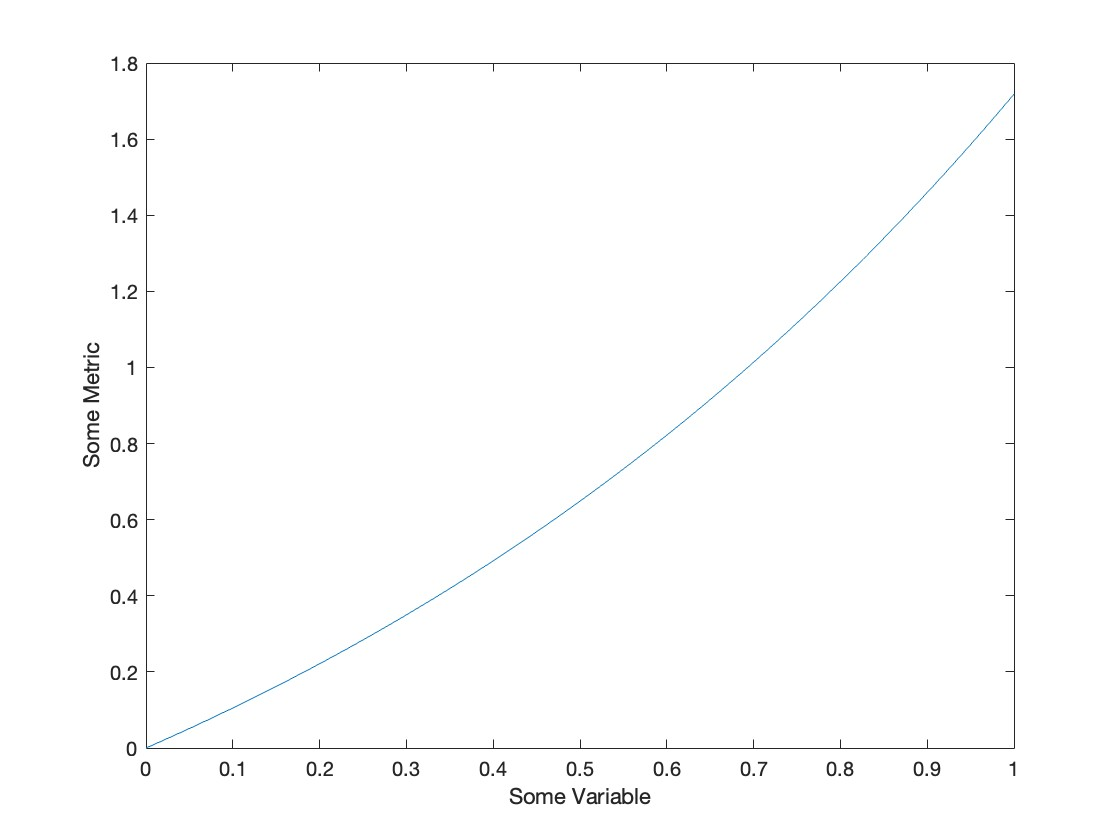
\includegraphics[width=0.65\textwidth]{Images/a_graph.jpg}
            \caption{A bad JPEG graph exported from MATLAB.}
            \label{fig:BadGraph}
        \end{figure}
    
        When you make plots in MATLAB make sure you export them as EPS images and that the text and lines are of sufficient size to be seen in the final document, as in \Cref{fig:BetterGraph}.

        \begin{figure}[ht!]
            \centering
            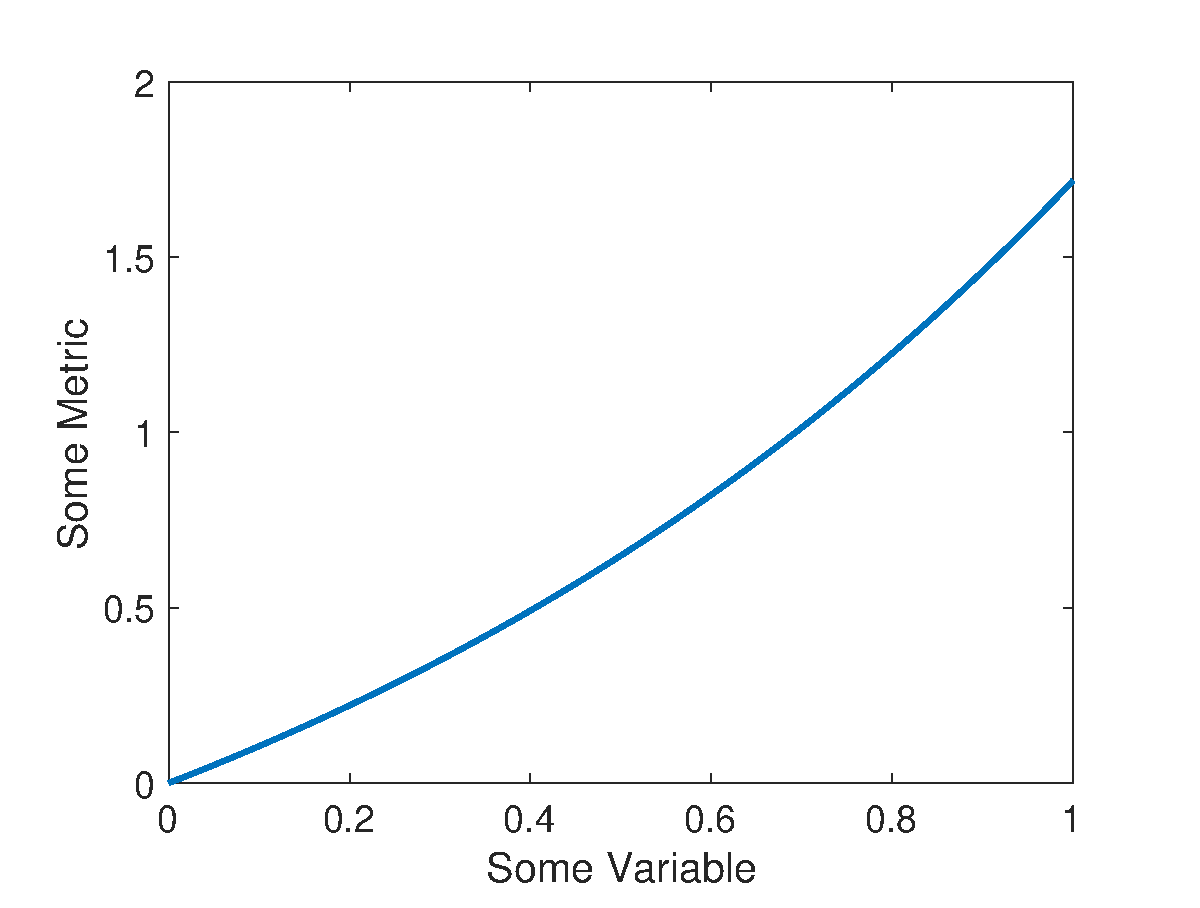
\includegraphics[width=0.65\textwidth]{Images/a_graph.eps}
            \caption{A better EPS graph exported from MATLAB.}
            \label{fig:BetterGraph}
        \end{figure}
    
    \subsection{Tables}
    \label{sec:Tables}
        You quite often need to limit the width of tables in your document. Latex provides the paragraph column type for this. But if you want things centre aligned you can use the additional column type provided by this template. See \Cref{tab:ColumnTypes} for a demonstration.
    
        \begin{table}[ht!]
            \centering
            \begin{tabular}{|p{4cm}|C{4cm}|}
                \hline
                The `p' column type produces a left aligned paragraph of the given width. & The `C' column type does the same but centre aligned. \tabularnewline
                \hline
            \end{tabular}
            \caption{Defining the width of table columns.}
            \label{tab:ColumnTypes}
        \end{table}
    
        There are several other fancy packages for doing tables in latex, so have a look around for what you need.

\end{appendices}

\end{document}